\section{Interfaces and Program Semantics}
\label{app:protocol}

The current interface is a complete environment program, not a mandatory World--Scene stack. A module-level \code{build()} returns an \code{Environment}. Its sampler generates all initial data and goals before rollout; an \code{Episode} owns each rollout's independent mutable state. Generated modules are not imported on the host as part of paper preparation.

\begin{table}[ht]
\centering\small
\caption{Responsibilities of a reusable environment program.}
\label{tab:interface}
\begin{tabularx}{\linewidth}{@{}lX@{}}
\toprule
Interface & Responsibility\\
\midrule
\code{make\_task(seed, parameters)} & Deterministically return a request and JSON payload.\\
\code{start(task)} & Create fresh episode state and actor-visible instructions.\\
\code{@tool(..., actor=...)} & Declare matching schemas and executable methods.\\
\code{available(name, actor)} & Define dynamic actor-specific visibility.\\
\code{next\_user / user\_context} & Supply scripted follow-ups or legitimate model-backed user context.\\
\code{check(task, state, trace)} & Evaluate requested outcomes from actual state and execution.\\
\code{validate(reference)} & Assert selected tool/reward behavior, including meaningful rejection cases.\\
\bottomrule
\end{tabularx}
\end{table}

Task serialization binds the program-bank digest, request, payload, sampling parameters, and an initial signature covering state, public instructions, visible tools and user context. Repeated sampling with identical inputs must agree. Episode state is copied; expected tool rejection restores the previous state and records the result. These checks are consistency safeguards, not a proof that arbitrary Python or all unseen task instances are correct.

\paragraph{Reward.}
A generated task returns a Boolean or programmatic \code{Score}. With outcome components $c_k\in[0,1]$, mandatory guards $g_\ell\in\{0,1\}$ and positive pre-fixed weights $w_k$,
\begin{equation}
R_x(\tau)=\left(\prod_\ell g_\ell\right)
\frac{\sum_k w_k c_k}{\sum_k w_k},
\qquad
\operatorname{Success}_x(\tau)=
\ind[\forall k:c_k=1\ \land\ \forall\ell:g_\ell=1].
\label{eq:score}
\end{equation}
The broader framework contains optional semantic-rubric support, but the studied task-generation contract excludes it. Model-backed users and independent solvability reviewers remain distinct from programmatic training rewards. Official target graders retain their own scoring logic.

\paragraph{Bounded checks.}
Changed programs undergo CPU execution checks and a model review of up to three representative constructed instances (first, middle, last), not an exhaustive semantic audit. At most one code repair is permitted. Retention can reuse the accepted review when code and sampler parameters match; all new tasks still receive executable checks. Promotion checks that request, payload, initial signature and sampling semantics remain unchanged. Failed candidates and exact duplicates produce explicit shortfalls, with no unplanned backfill.

\section{Study Versions and Evidence Boundaries}
\label{app:versions}

The earlier manuscript described World--Scene interfaces, curated World initialization and a separate student probe. Those describe a superseded protocol, not the results reported here. The three selected runs use \code{persistent\_environment\_v5}; their initial Git trees contain only an empty-bank seed manifest under \code{env/}. Generic interface examples remain provided.

\begin{table}[ht]
\centering\small
\caption{Frozen study identities and important differences. These are separate runs, not matched ablation arms.}
\begin{tabularx}{\linewidth}{@{}p{.28\linewidth}>{\raggedright\arraybackslash}X>{\raggedright\arraybackslash}X>{\raggedright\arraybackslash}X@{}}
\toprule
 & $\tau^2$ & BFCL & ACEBench-Agent\\
\midrule
Run suffix & \code{83b860} & \code{defa84} & \code{22571a}\\
Launch (Beijing time) & Sep.\ 13, 02:25 & Sep.\ 13, 02:25 & Sep.\ 14, 09:46\\
Snapshot rounds & 9, stopped & 9, stopped & 10, stopped\\
Test checkpoints & R1--R9 & R1--R9 & R1--R10\\
Task bank at start & Empty & Empty & Empty\\
Expectation/review contract & Earlier v5 & Earlier v5 & Decision brief v1\\
RL feedback access & Earlier diagnostic views & Earlier diagnostic views & Full group queries\\
Pods per training job & 2 & 2 & 4\\
Recorded episode aborts & 2/6,768 & 33/6,472 & 0/5,008\\
\bottomrule
\end{tabularx}
\end{table}

The shared base model is Qwen3-4B-Instruct-2507, with RL temperature 0.7, 65,536-token context, 16,384-token response cap, task-group size eight, learning rate $3\times10^{-6}$, and fixed-reference KL coefficient 0.005. The recorded optimizer seed is 1234. Up to eight Tasks form one update; smaller tails are kept. The controller task configuration limits interactions separately from benchmark evaluation. Program construction is CPU work; pod counts refer to leased GPU jobs, with four GPUs per pod.

Recorded complete rounds report weight changes, finite training metrics, complete policy-token capture and task-group reward normalization. This does not make their training data defect-free: aborted episodes remain part of the audit, and maintenance/restart history is retained. No cancelled attempt or archived alternative checkpoint is substituted into a completed-round curve. The final confirmatory study should rerun a frozen, matched protocol with independent seeds.

Direct inspection of the retained rollout archives attributes 32 BFCL R2 aborts to an invalid model-backed user-context contract and one BFCL R1 abort to an empty user turn. The two $\tau^2$ aborts are a user-tool interaction-budget exhaustion in R3 and an empty user turn in R8. These are not ordinary failed task outcomes or evidence that a task was simply too difficult. They qualify the historical training studies even though their subsequent fixed-target evaluations completed.

\subsection{Benchmark Protocols}

\paragraph{$\tau^2$-Bench.}
Each half has 25 airline, 57 retail and 57 telecom tasks. The revised fixed-seed partition stratifies airline/retail business-action labels and telecom issue/persona labels. Its baseline was repartitioned from existing real evaluations without resampling responses; some earlier test-side records required reconstruction of static tool/schema wrappers, which is disclosed in their provenance. Overall is task-weighted, not an unweighted mean of domains. The evaluation policy is greedy and the user is GPT-5.4 at temperature zero.

Checkpoint test evaluation uses a replay repair that preserves the live behavior of unknown/rejected tools instead of allowing an exception to abort final-state reconstruction. Accepted test records use the corrected judge configuration and replay-v2 lineage; failed and superseded v1 evaluations are excluded. The historical test baseline predates the replay repair and is explicitly marked non-comparable in the dashboard registry. Figure~\ref{fig:evolution} connects it for visual continuity and shows the stored-score difference; this is not a matched-protocol gain. Table~\ref{tab:main} omits its gain estimate and paired interval.

\paragraph{BFCL.}
The fixed dev/test halves contain 100 tasks each from Base, Long Context, Missing Function and Missing Parameter. Legacy framework identifiers such as \code{bfcl\_v3} are adapter names, not evidence that a full leaderboard suite was evaluated. The matched test base comes from the recorded September 6 collection with the same task membership, model, repeats and evaluation/serving configuration. The paper reports only these four multi-turn subsets.

\paragraph{ACEBench-Agent.}
The English Agent release is pinned to official source revision \code{56dd66c}. Its 20 multi-step and 30 multi-turn tasks are split by category and tool-class strata into equal dev/test halves (10+15 each), with seed 1234. We report the unweighted mean of the two category scores, matching the metric definition used in SPADE, not its complete evaluation protocol.

The studied run uses \code{acebench\_native\_fc\_v1}: native structured tool calls and full append-only assistant/tool history, with the native business tools, task initialization, GPT-5.4 user, 40-event budget and official end-state grading. The audited schema projection corrects the documented required-field typo for \code{reserve\_flight}; malformed arguments are not repaired to make episodes succeed. The 4B policy uses temperature 0.001 and a 1,000-token output budget. Multi-step outer prompts retain the wrapper's Chinese compatibility setting while tasks/tools remain English; multi-turn prompts are English. These transport, history, user-model and serving details preclude presenting the scores as an exact SPADE reproduction.

The older September 13 ACE textual-interface study is not spliced into the native-FC curve. Its archived alternate training attempt is also excluded. Native test measurements cover all ten completed checkpoints. The later sweep reuses R1--R4 results and adds R5--R10 on the same 25 test tasks with three repeats and the same native-FC protocol. R6/R8 initially failed during remote toolchain detection before inference; the completed recovery results are included and the failed-start records are retained in provenance. Training was stopped during R11, which has no registered complete checkpoint and is excluded.

\subsection{Snapshot and Statistical Construction}

The original snapshot at 14 September 2026, 16:04:42 UTC remains unchanged. A supplementary snapshot at 17:43:25 UTC (15 September 01:43:25 Beijing time) adds ACE R5--R10 test results and R10 development/training records. It retains the other two studies exactly, yielding nine completed rounds each for $\tau^2$/BFCL and ten for ACE. All included checkpoints have test results. Rebuilding the paper does not query or update source experiments.

Each plotted evaluation was independently recounted from stored per-task three-repeat outcome groups and checked against saved summary metrics. The updated snapshot records 218 source-file hashes, the prior snapshot's hash, run/job/revision identities, actual task allocations, training audit fields, and links to baseline and operator-only test collections. The update checks that earlier ACE measurements and training records are unchanged; new test records match registered checkpoints and retain the fixed task membership. It contains outcome summaries, not a new evaluation. The paper scripts neither import generated environment modules nor invoke training, serving, grading or controller actions.

Selection uses the earliest maximum dev mean over R0 and the included completed checkpoints, with numerical ties rounded to twelve decimal places. It is an explicitly applied analysis rule, not a claim of preregistration. For paired test differences, each bootstrap draw samples tasks with replacement within their fixed subset, retains all three repeats for each sampled task, and applies the original aggregation: task-weighted for BFCL and a two-category macro mean for ACE. We use 10,000 draws with bootstrap seed 20260914. The $\tau^2$ baseline mismatch excludes its paired baseline comparison.

\section{Within-Benchmark Evolution}
\label{app:subsets}

\begin{figure}[ht]
\centering
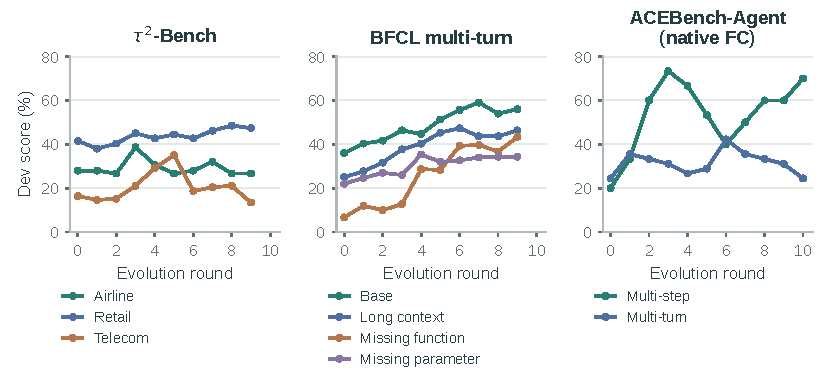
\includegraphics[width=\linewidth]{figures/subsets.pdf}
\caption{Fixed development-subset trajectories. These use the benchmark's fixed labels, not the Planner's changing analysis-domain names. BFCL's Missing Function subset improves substantially; the later $\tau^2$ decline is particularly visible in Telecom. Native ACE's early gain is concentrated in Multi-Step. The figure describes associations within the recorded runs, not attribution to a particular environment revision.}
\label{fig:subsets}
\end{figure}

\section{Confirmatory Comparisons Still Needed}
\label{app:ablations}

\begin{table}[ht]
\centering\small
\caption{Unmeasured controls; no synthetic scores are supplied.}
\begin{tabularx}{\linewidth}{@{}lX@{}}
\toprule
Control & Question isolated\\
\midrule
Fixed library, fresh Tasks & Does later research improve over resampling and training alone?\\
Sampler/allocation only & Does executable program revision add value?\\
No maintained experience & Does accumulated, corrected research experience help?\\
Stale target evidence & Does fresh behavioral feedback change useful decisions?\\
No stable requirement map & Does explicit task-linked coverage improve retention or targeting?\\
Whole-program generation without persistence & Does retaining and revising assets improve cost or transfer?\\
\bottomrule
\end{tabularx}
\end{table}

Controls should share model initialization, target-information access and evaluation protocols. Compare both matched training episodes and matched total research budgets; count failed implementations, reviewer requests and all serving/evaluation overhead. Additional evidence should include independently audited accepted and rejected tasks, one traced intervention from source case to code change and subsequent outcomes, and repeated evolution seeds. Independent test tasks reserved after method freeze are needed for a final confirmatory result.
